\chapter{Fermion Signs and Supersymmetric Cancellations}

\lectureoverview{Supersymmetry relates bosons to fermions, but the reason for wanting such a relation is easier to see before writing its algebra. We begin with the topology of rotations, make the sign of a fermion wavefunction observable through interference, derive the minus sign of a closed fermion loop from exchange antisymmetry, and then use the opposite bosonic and fermionic loop signs to motivate cancellations of vacuum energy and scalar self-energy. The second half asks how badly supersymmetry may be broken, how one might detect superpartners, and why exact supersymmetry would erase ordinary atomic shell structure.}

\section{Before Supersymmetry: A Peculiarity of Rotations}

Supersymmetry is a symmetry between fermions and bosons. Before trying to construct it, however, it is worth recalling how differently these two kinds of particles respond to rotations. That question itself begins with a topological fact that is easy to demonstrate and surprisingly difficult to forget once one has seen it.

Hold one hand palm upward and rotate the wrist through \(2\pi\). The hand returns to its original orientation, but the arm plainly has not returned to an equivalent configuration: it is twisted. Continue through another \(2\pi\), moving the arm around as necessary, and the twist can be removed. Thus a \(2\pi\) rotation is not continuously deformable to no rotation while the surroundings are held fixed, whereas a \(4\pi\) rotation is. The hand demonstration is a proof by hand-waving in the most literal sense.

The same point can be made without relying on anatomy. Put a ball in a fixed box and attach the ball to the walls with any number of flexible, stretchable, but unbreakable strings. Rotate the ball once through \(2\pi\). The strings become tangled, and no motion of the strings alone restores the original configuration. Rotate the ball through a total angle \(4\pi\), and the strings can be carried around it until the tangle disappears. The walls stand for spatial infinity: the comparison is meaningful only because the boundary is not rotated along with the ball.

\begin{classroomqa}
\audiencequestion{Could the tangle be removed by rotating the box? \lecturetimestamp{00:02:53}}
\lecturerresponse{That changes the problem. The box represents spatial infinity and is held fixed. We are comparing a rotation of the object relative to its surroundings, not a common rotation of object and surroundings.}
\end{classroomqa}

\begin{classroomqa}
\audiencequestion{Why not simply rotate the ball by another \(2\pi\)? \lecturetimestamp{00:03:20}}
\lecturerresponse{That is precisely what distinguishes the two cases. Without rotating the ball further, the tangle left by one \(2\pi\) turn cannot be removed. After the second turn, giving a total of \(4\pi\), it can.}
\end{classroomqa}

In modern group language, the rotation group has two topological classes of closed paths:
\begin{equation}
\pi_1\!\left(SO(3)\right)\cong \mathbb Z_2.
\end{equation}
A single traversal is nontrivial, but traversing twice gives the trivial class.
Equivalently, \(SU(2)\) is the double cover of \(SO(3)\). This is the geometric
prehistory of the fermion sign.

\editorialnote{The language of \(SO(3)\), \(SU(2)\), and the fundamental group
makes the topology explicit. The arm demonstration and the string demonstration
establish the same two-valued behavior geometrically.}

\section{What a \texorpdfstring{\(2\pi\)}{2 pi} Rotation Does to a Quantum State}

Now nail down the position of a particle and retain only its spin state, denoted by \(\ket{\psi}\). Integer-spin particles are bosons and half-integer-spin particles are fermions. A physical rotation can be implemented by putting a charged spin in a strong magnetic field and rotating the field, or by allowing the spin to precess through the desired angle in a fixed field.

\begin{classroomqa}
\audiencequestion{How can an electron spin actually be rotated in the laboratory? \lecturetimestamp{00:05:26}}
\lecturerresponse{A magnetic field supplies the handle. One may rotate a sufficiently strong field so that the spin follows it, or let the spin precess around a fixed field. Grabbing the electron by hand is not a competitive experimental method.}
\end{classroomqa}

Suppose a full \(2\pi\) rotation multiplies the state by a phase:
\begin{equation}
R(2\pi)\ket{\psi}=\xi\ket{\psi}.
\end{equation}
Performing the operation twice gives
\begin{equation}
R(4\pi)\ket{\psi}=\xi^2\ket{\psi}.
\end{equation}
Since the \(4\pi\) path is topologically trivial, it must act as the identity in this comparison. Therefore
\begin{equation}
\xi^2=1,
\qquad
\xi=+1\ \hbox{or}\ -1.
\end{equation}
Bosons realize the plus sign and fermions the minus sign:
\begin{align}
R(2\pi)\ket{\psi_B}&=+\ket{\psi_B},\\
R(2\pi)\ket{\psi_F}&=-\ket{\psi_F}.
\end{align}
For a state of definite spin \(j\), the compact statement is
\begin{equation}
R(2\pi)=(-1)^{2j}.
\end{equation}
The transcript briefly says that the second possibility is multiplication by \(2\pi\); the surrounding derivation and the board argument make clear that the intended factor is \(-1\).

At first this seems physically empty. If an entire wavefunction changes sign,
\begin{equation}
\Psi\longmapsto-\Psi,
\end{equation}
then probabilities are unchanged because
\begin{equation}
(-\Psi)^*(-\Psi)=\Psi^*\Psi.
\end{equation}
Take two ensembles of identically prepared electrons, rotate every member of one ensemble by \(2\pi\), and leave the other ensemble alone. No measurement on an isolated member can reveal which ensemble it came from. An overall phase is not an observable.

\section{Making the Minus Sign Relative}

The sign becomes observable when it is imposed on one coherent branch of a wavefunction but not the other. Send electrons one at a time through a two-path apparatus. Do not determine which path is taken, because which-path information destroys interference. Let the upper and lower amplitudes be \(\psi_1\) and \(\psi_2\), so that the recombined state is
\begin{equation}
\Psi=\psi_1+\psi_2.
\end{equation}
Imagine temporarily trapping each branch in a magnetic region. Rotate only the field associated with the second branch through \(2\pi\). If the particle is a fermion, the state becomes
\begin{equation}
\Psi'=\psi_1-\psi_2.
\end{equation}
This is no longer a global sign. The relative phase shifts interference maxima into minima. If the two returning packets are mirror images about the middle of the detector, the antisymmetric combination vanishes at the center:
\begin{equation}
\Psi'(0)=\psi_1(0)-\psi_2(0)=0.
\end{equation}
The electron is therefore never detected at that symmetry point. Rotating both branches would instead produce \(-\psi_1-\psi_2=-\Psi\), which has no observable effect.

The lecture emphasizes the relational nature of the experiment. Rotating one magnetic region relative to the other is analogous to rotating the ball while holding the box fixed. Rotating both regions together is analogous to rotating ball and box together. A relative \(4\pi\) rotation removes the effect because the fermion state then returns with a plus sign. The experiment was proposed by Yakir Aharonov and Leonard Susskind in 1967 and was later realized in interferometric form, as the lecture notes in passing. The same principle can be applied to electrons or charged ions: a shifted fringe pattern identifies a half-integer-spin state, while an unshifted pattern identifies an integer-spin state.

\begin{classroomqa}
\audiencequestion{If the relative field is rotated through \(4\pi\), does the shifted pattern return to the original one? \lecturetimestamp{00:12:21}}
\lecturerresponse{Yes. Two sign changes multiply to \(+1\), so the relative phase responsible for exchanging maxima and minima disappears.}
\end{classroomqa}

\begin{classroomqa}
\audiencequestion{How literally should the strings in the box be associated with a fermion? \lecturetimestamp{00:13:43}}
\lecturerresponse{They are a topological mnemonic, not physical strings attached to an electron. A boson behaves as though a \(2\pi\) turn leaves no memory; a fermion retains precisely the sign memory represented by the nontrivial tangle.}
\end{classroomqa}

\begin{classroomqa}
\audiencequestion{Are there two electrons in the two magnetic regions, one rotated and one not? \lecturetimestamp{00:14:29}}
\lecturerresponse{No. There is one electron in a coherent spatial superposition. It has an amplitude to occupy either branch, and the apparatus must not reveal which branch it occupied. Rotating one region changes one amplitude relative to the other; rotating both changes only the common phase.}
\end{classroomqa}

The angle \(2\pi\) is special because the spin orientation returns to itself while the spinor acquires a sign. A generic relative rotation changes the spin orientation as well. If the two path states return with spin states \(\ket{\chi_1}\) and \(\ket{\chi_2}\), the interference term is proportional to
\begin{equation}
\braket{\chi_1}{\chi_2}.
\end{equation}
Its magnitude controls fringe visibility.\editorialnote{The spin-overlap formula is a standard completion of the lecture's qualitative discussion of partial and complete loss of interference.} Orthogonal spin states carry perfect which-path information and do not interfere.

\begin{classroomqa}
\audiencequestion{What happens if one measures which magnetic region contained the electron? \lecturetimestamp{00:18:03}}
\lecturerresponse{The interference pattern is destroyed. Any record that distinguishes the two paths removes the coherent addition of their amplitudes.}
\end{classroomqa}

\begin{classroomqa}
\audiencequestion{If all spins begin in the same direction and the final spin is measured, does the \(2\pi\) operation itself change that direction? \lecturetimestamp{00:18:17}}
\lecturerresponse{No. After \(2\pi\) the physical spin direction is the same; only the fermionic branch has acquired a minus sign. That is why this operation can change interference without leaving a different spin orientation as a path marker.}
\end{classroomqa}

\begin{classroomqa}
\audiencequestion{What if the field is turned only through \(\pi\), rather than \(2\pi\)? \lecturetimestamp{00:18:43}}
\lecturerresponse{Then the spin direction changes. An up-spin branch and a down-spin branch are distinguishable and cannot interfere. Intermediate angles reduce the visibility continuously; a \(180^\circ\) relative turn destroys it completely.}
\end{classroomqa}

\section{Exchange Symmetry and the Sign of a Closed Loop}

The rotation discussion has isolated one fermionic minus sign. A second, closely related sign appears when identical particles are exchanged. For a two-particle wavefunction,
\begin{align}
P_{12}\Psi_B(1,2)&=+\Psi_B(1,2)=+\Psi_B(2,1),\\
P_{12}\Psi_F(1,2)&=-\Psi_F(1,2)=-\Psi_F(2,1).
\end{align}
Bosonic states are symmetric and fermionic states antisymmetric.

\begin{figure}[htbp]
\centering

\includegraphics[width=0.74\textwidth]{lecture_02_figure_02.png}
\lectureframe{00:24:27}
\caption{The exchange argument in state notation. Only the ket label is securely legible in the frame; the antisymmetry equations are typed in the text rather than attributed to obscured chalk.}
\end{figure}

We can now determine the relative sign of a closed particle loop without evaluating its integral. Consider a vacuum Feynman diagram with no external legs. It may be pictured as a particle tracing a closed path in spacetime, or as a particle-antiparticle pair being created and later annihilated. Such a vacuum diagram contributes to the vacuum amplitude and hence to the vacuum energy.

Start with two disconnected copies of the loop. Disconnected diagrams multiply, so if one loop has sign \(\sigma\), the pair has sign
\begin{equation}
\sigma^2=+1.
\end{equation}
Cut both loops at a common time, say \(t=0\). At that slice there are two identical particles. Reconnect them without exchange and the two separate loops return. Exchange the two particles before reconnecting and the topology becomes one loop. The exchange contributes \(+1\) for bosons and \(-1\) for fermions. Since the starting two-loop sign was positive, the resulting one-loop signs are
\begin{equation}
\begin{aligned}
\operatorname{sign}(\text{closed boson loop})&=+1,\\
\operatorname{sign}(\text{closed fermion loop})&=-1.
\end{aligned}
\end{equation}
More generally, a diagram with \(L_F\) independent closed fermion loops carries the factor
\begin{equation}
(-1)^{L_F}.
\end{equation}
The lecture deliberately derives this rule from exchange rather than invoking Grassmann integration. The elementary argument makes the physical origin of the sign visible.

\section{Opposite Loop Signs and Vacuum Energy}

A bosonic vacuum loop raises the vacuum contribution with one sign, while a fermionic loop enters with the opposite sign. This is immediately suggestive because the observed dark-energy density is extremely small compared with naive cutoff estimates in quantum field theory. The lecture quotes the notorious discrepancy as roughly \(123\) orders of magnitude. The precise exponent depends on which ultraviolet scale is used; the durable point is the fantastic mismatch.

The value of a loop depends on more than statistics. It depends on mass, charge, multiplicity, and interactions. Yet if a boson and fermion match in all relevant properties, their equal-magnitude contributions can cancel:
\begin{equation}
\begin{gathered}
m_B=m_F,\qquad q_B=q_F,\qquad g_B=g_F,\\
\Delta\rho_{\mathrm{vac}}^{(B)}
+\Delta\rho_{\mathrm{vac}}^{(F)}=0.
\end{gathered}
\end{equation}
This observation does not solve the cosmological-constant problem. It merely supplies something that ordinary bosonic loops alone could not supply: contributions of the opposite sign. In an exactly unbroken globally supersymmetric theory, vacuum-energy cancellations can indeed be exact under the appropriate assumptions; after supersymmetry is broken, the observed tiny nonzero value remains unexplained.\editorialnote{This qualification separates the lecture's motivation from the much harder cosmological-constant problem.}

Exact matching is already known not to describe nature. If the electron had a spin-zero partner with the same mass and electric charge, electron-positron annihilation through a virtual photon could produce a pair of them:
\begin{equation}
e^-e^+\longrightarrow\gamma^*
\longrightarrow\widetilde e^-\widetilde e^+.
\end{equation}
A degenerate charged scalar would not have escaped ordinary collider experiments. Thus the boson-fermion reflection cannot be an exact symmetry of the observed spectrum. This is a reflection in particle type, not a reflection in physical space.

\section{The More Immediate Target: Scalar Self-Energy}

Vacuum energy is the first illustration, but the lecture's main concern is the radiative instability of scalar masses. A scalar that begins with zero bare mass can receive a quadratically cutoff-sensitive correction. Schematically,
\begin{equation}
\Delta m_H^2\sim \frac{g_B^2}{16\pi^2}\Lambda^2
\end{equation}
from a bosonic loop. Fermion masses have a different protection: when a massless fermion has an exact chiral symmetry, radiative corrections cannot generate an additive mass term. That was the left-right argument of the preceding lecture.

Now imagine a symmetry rigid enough to place a scalar and a fermion in one multiplet and to match their interactions. A fermion loop then appears with the opposite sign:
\begin{equation}
\Delta m_H^2
\sim
\frac{g_B^2-g_F^2}{16\pi^2}\Lambda^2+\cdots .
\end{equation}
If supersymmetry enforces \(g_B=g_F\) and equal masses, the quadratic terms cancel. The fermion's protection is thereby transmitted to its bosonic partner. This is not merely a numerical coincidence between two diagrams; the symmetry must enforce the cancellation through every order and every allowed interaction.

The broad blackboard comparison shows the lecture moving from isolated loops to paired loop corrections of propagating particles.

\begin{figure}[htbp]
\centering

\includegraphics[width=0.79\textwidth]{lecture_02_figure_04.png}
\lectureframe{00:40:23}

\medskip
\begin{tikzpicture}[scale=0.9]
\draw (-4.2,0) circle (0.55);
\draw[dashed] (-2.4,0) circle (0.55);
\draw (0,0) -- (3.7,0);
\fill (1.85,0) circle (0.055);
\draw (1.85,0) -- (1.85,0.25);
\draw[dashed] (1.85,0.85) circle (0.6);
\end{tikzpicture}
\caption{A board-wide comparison of ordinary and partner loop topologies. The typed sketch preserves only the visible topological contrast; it does not assign obscured particle labels.}
\end{figure}

After the classroom break, the argument restarts with what is called the zeroth-order picture. This is not an order in perturbation theory. It means the roughest useful account:
\begin{quote}
For every particle there is a superpartner of the opposite statistics. Every fermion has a bosonic partner, and every boson has a fermionic partner.
\end{quote}
In an exact supersymmetric theory the partners would also be degenerate, meaning equal in mass. Nature is not degenerate in this way. Still, if the masses are unequal but not too far apart, the cancellation may remain good enough to prevent an explosively large scalar correction. With soft supersymmetry breaking, the dangerous scale is replaced schematically by the superpartner splitting:
\begin{equation}
\Delta m_H^2\sim
\frac{g^2}{16\pi^2}\,\Delta m_{\mathrm{SUSY}}^2
\ln\!\frac{\Lambda^2}{\Delta m_{\mathrm{SUSY}}^2}
\end{equation}
up to model-dependent coefficients.\editorialnote{This formula expresses the lecture's qualitative statement that imperfect mass matching leaves a residual correction controlled by the splitting; it is not copied from the board.}

\section{Broken Supersymmetry and the 2010 Experimental Bet}

No superpartner had been observed when this lecture was recorded in 2010. The immediate inference was that the partners, if real, must be heavier than the known particles and heavier than the reach of earlier machines. Supersymmetric models also distinguish particles whose masses arise only after electroweak symmetry breaking from states allowed to carry larger symmetry-preserving masses. The lecture offers this as a rationale for why the visible half of a supersymmetric spectrum might be light while the unseen half is heavier, while candidly calling the arrangement a stretch. Susskind states his own expectation that superpartners would be detected, then immediately marks it as a guess rather than a result.

The Large Hadron Collider was therefore central to the lecture's outlook. It was expected to search both for the Higgs boson and for superpartners. These statements must be read in their 2010 setting: the lecture is explaining the experimental bet before the Higgs discovery and before later LHC search results.

Why should a naturalness-motivated superpartner not sit at the Planck scale? Because it would then fail at the task assigned to it. If the boson and fermion masses differ enormously, their loop integrals cease to cancel above the lighter mass. The residual scalar correction is set roughly by the heavy splitting rather than by the weak scale. Supersymmetry at an arbitrarily remote scale is still a mathematical symmetry, but it no longer gives a persuasive explanation for a light Higgs sector.

The lecture translates this into its era's expectation that the relevant splittings should lie within roughly a few hundred GeV and hence within LHC reach. That numerical estimate is historical and model-dependent; the logical chain is more important:
\begin{equation}
\begin{gathered}
\text{Higgs protection}\\
\Downarrow\\
\text{effective boson--fermion cancellation}\\
\Downarrow\\
\Delta m_{\mathrm{SUSY}}\ \text{not too large}.
\end{gathered}
\end{equation}

\begin{classroomqa}
\audiencequestion{Could all fermionic contributions merely cancel all bosonic contributions in the aggregate, without one-to-one partners? \lecturetimestamp{00:45:01}}
\lecturerresponse{They could cancel numerically, but that would be an accidental cancellation as finely tuned as the original problem. The supersymmetric proposal is stronger: reasonable postulates enforce matched contributions, while broken supersymmetry explains why the masses are only approximately matched. Vacuum energy was the illustration; the immediate concern here is the Higgs self-energy.}
\end{classroomqa}

\begin{classroomqa}
\audiencequestion{Is calling an aggregate cancellation unnatural already assuming a reductionist way of organizing the theory? \lecturetimestamp{00:47:51}}
\lecturerresponse{That is a fair challenge. Nobody has a final definition of naturalness, and the search is partly a matter of groping for a compelling explanation. Supersymmetry and spontaneous supersymmetry breaking provide known mathematical frameworks that can enforce the desired pattern. The unresolved questions are whether nature uses that framework and whether it is unique.}
\end{classroomqa}

\section{Direct Production, Virtual Effects, and Decay Chains}

A heavy particle need not be produced on shell to influence an experiment. It can occur virtually inside a loop and slightly modify an ordinary electron-positron scattering amplitude. Precision electroweak measurements therefore constrain superpartners even when the center-of-mass energy is below the direct pair-production threshold
\begin{equation}
\sqrt{s}<2m_{\widetilde p}.
\end{equation}
The lecture's 2010 assessment is that precision data were already squeezing supersymmetric parameter space but had not ruled it out.

\begin{classroomqa}
\audiencequestion{Could superpartners be inferred indirectly, as earlier heavy particles were constrained through precise production rates before direct observation? \lecturetimestamp{00:49:01}}
\lecturerresponse{Yes. A virtual superpartner loop changes an ordinary amplitude slightly, so the problem becomes high-precision electroweak phenomenology rather than direct production. A clean, sufficiently energetic electron-positron collider would be especially useful. Proton collisions are messier because a proton is a composite state of quarks and gluons; one is really colliding fluctuating constituents, not two elementary particles with sharply known initial conditions.}
\end{classroomqa}

One student asks about running the reaction in reverse, beginning with abundant superparticles. The obstacle is not time-reversal symmetry but availability. Heavy superpartners must first be created, and most are expected to decay rapidly into lighter states.

\begin{classroomqa}
\audiencequestion{If a universe contained many superparticles, could two of them collide and turn into ordinary particles? \lecturetimestamp{00:53:43}}
\lecturerresponse{In principle the relevant reactions have reverse channels, but heavy superpartners are not expected to remain freely abundant. They decay toward lower-energy states, so an experiment must first supply enough collision energy to create them.}
\end{classroomqa}

This raises the dark-matter question. In many supersymmetric models a discrete selection rule prevents the final superpartner in a decay chain from disappearing entirely. Then every heavier superpartner cascades toward the lightest superpartner, or LSP. If the LSP is electrically neutral, it can be stable and difficult to detect, making it a possible dark-matter candidate. The transcript once says "dark energy" in this exchange, but the audience's question and the particle description unambiguously concern dark matter.

\begin{classroomqa}
\audiencequestion{Does rapid superpartner decay conflict with the proposal that a superpartner could be dark matter? \lecturetimestamp{00:54:53}}
\lecturerresponse{No. Most superpartners may decay while the lightest one remains stable in models that require a superpartner at the end of each decay chain. Electric charge generally raises additional phenomenological difficulties, so the viable LSP is likely neutral. It is not undetectable in principle, but it would not leave the obvious ionizing track of a charged selectron.}
\end{classroomqa}

\section{Matching Means Matching the Couplings}

Mass matching alone is insufficient. Compare an electron vacuum loop with a selectron loop. Their opposite statistics supply opposite signs, but equal magnitudes require equal masses. Now attach two external photons. The coefficients also contain the electric couplings, so cancellation requires equal charges:
\begin{equation}
\begin{gathered}
q_{\widetilde e}=q_e,\\
\mathcal A_{\mathrm{loop}}^{(e)}
+\mathcal A_{\mathrm{loop}}^{(\widetilde e)}=0,\\
\text{provided the full couplings match.}
\end{gathered}
\end{equation}
A mismatch at any level leaves an uncancelled divergent term. Supersymmetry is valuable because it relates interactions as well as names and spins.

\begin{figure}[H]
\centering

\includegraphics[width=0.66\textwidth]{lecture_02_figure_05.png}
\lectureframe{00:57:15}

\medskip
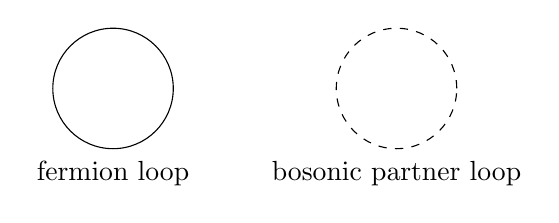
\begin{tikzpicture}[scale=0.9]
\draw (-2.0,0) circle (0.85);
\draw[dashed] (2.0,0) circle (0.85);
\node at (-2.0,-1.2) {fermion loop};
\node at (2.0,-1.2) {bosonic partner loop};
\end{tikzpicture}
\caption{Solid and dashed loops compared during the charge-matching argument. The cropped external marks are not reconstructed because the frame alone does not determine every attachment.}
\end{figure}

\begin{classroomqa}
\audiencequestion{Could superpartners have escaped detection simply because their coupling constants are different? \lecturetimestamp{00:56:23}}
\lecturerresponse{Not if the same diagrams are to cancel. Adding photon interactions tests the electric charge of each line. Unequal couplings give unequal numerical loop factors and restore the large remainder. The symmetry must match the appropriate charges and interactions.}
\end{classroomqa}

\begin{classroomqa}
\audiencequestion{Should the photon's superpartner also be massless? \lecturetimestamp{00:58:01}}
\lecturerresponse{It would be massless in an exact supersymmetric theory because it would be degenerate with the photon. The observed world is not exactly supersymmetric, so a physical photino-like state need not share the photon's mass.}
\end{classroomqa}

\section{The Superpartner Dictionary}

The naming rules are inelegant but useful. A boson receives a fermionic partner whose name often ends in \emph{-ino}: photon and photino, the \(W\) and wino, the \(Z\) and zino, gluon and gluino, Higgs and Higgsino, graviton and gravitino. An ordinary fermion receives a bosonic partner whose name usually begins with \emph{s-}: electron and selectron, quark and squark.

\begin{center}
\begin{tabular}{@{}>{\raggedright\arraybackslash}p{0.40\linewidth}>{\raggedright\arraybackslash}p{0.52\linewidth}@{}}
\toprule
ordinary state & superpartner and spin change\\
\midrule
scalar Higgs, \(j=0\) & Higgsino, \(j=\tfrac12\); \(\Delta j=+\tfrac12\)\\
gauge boson, \(j=1\) & gaugino, \(j=\tfrac12\); \(\Delta j=-\tfrac12\)\\
matter fermion, \(j=\tfrac12\) & sfermion, \(j=0\); \(\Delta j=-\tfrac12\)\\
graviton, \(j=2\) & gravitino, \(j=\tfrac32\); \(\Delta j=-\tfrac12\)\\
\bottomrule
\end{tabular}
\end{center}

The general relation is that members of a supermultiplet differ by half a unit of spin:
\begin{equation}
\Delta j=\frac12.
\end{equation}
The rough lecture examples pair a spin-\(\tfrac12\) matter fermion with a scalar and a spin-one gauge boson with a spin-\(\tfrac12\) gaugino. A complete interacting model can mix states after symmetry breaking, so the physical mass eigenstates need not retain these simplest names.

\begin{classroomqa}
\audiencequestion{Could all the new scalar partners undergo spontaneous symmetry breaking of their own? \lecturetimestamp{01:01:27}}
\lecturerresponse{Scalar fields can acquire expectation values, but arbitrary extra symmetry breaking would be phenomenologically disastrous. A viable supersymmetric model must arrange its scalar potential so that color, electric charge, and other required symmetries are not broken in the wrong way.}
\end{classroomqa}

\begin{classroomqa}
\audiencequestion{Does the Higgsino have special interactions corresponding to the Higgs quartic term? \lecturetimestamp{01:02:19}}
\lecturerresponse{Supersymmetry matches interactions as well as particles. The relation is not obtained by naively replacing every Higgs line with a Higgsino line, but the scalar quartic and the relevant fermionic and auxiliary interactions belong to one constrained structure. Those details have not yet been developed in the lecture.}
\end{classroomqa}

\begin{classroomqa}
\audiencequestion{Does the \(2\pi\)-versus-\(4\pi\) rotation theorem have analogues in other dimensions? \lecturetimestamp{01:03:07}}
\lecturerresponse{Yes, but dimensionality changes the possibilities. In two spatial dimensions exchange paths can wind around one another, allowing anyons whose exchange phases are more general than the bosonic \(+1\) and fermionic \(-1\). Such excitations occur in condensed-matter systems, but they are outside the present course's route.}
\end{classroomqa}

\section{Why Exact Supersymmetry Would Erase Chemistry}

We finally ask what an exactly supersymmetric world would be like. Exactness here means equal masses and matched interactions for every particle-superpartner pair. The electron would have a bosonic selectron with the same mass and electric charge, and the massless photon would have a massless fermionic photino:
\begin{equation}
m_{\widetilde e}=m_e,
\qquad
q_{\widetilde e}=q_e,
\qquad
m_{\widetilde\gamma}=m_\gamma=0.
\end{equation}

The familiar periodic structure of chemistry depends on Fermi statistics. Hydrogen has one electron in its lowest orbital. Helium accommodates two there because the spin labels differ. Lithium's third electron must occupy a higher orbital: the Pauli exclusion principle prevents three identical electrons from occupying the same one-particle state. That outer electron has more energy and would prefer to fall inward, ordinarily emitting a photon, but the filled lower states block the transition.

Exact supersymmetry opens another channel:
\begin{equation}
e^-_{\mathrm{outer}}
\longrightarrow
\widetilde e^-_{\mathrm{inner}}
+
\widetilde\gamma .
\end{equation}
The initial electron and emitted photino are fermions, while the remaining selectron is a boson. Because selectrons obey Bose rather than Fermi statistics, the final selectron is not excluded from an already occupied low orbital. The valence electron can therefore convert and fall inward.

\begin{figure}[H]
\centering

\includegraphics[width=0.62\textwidth]{lecture_02_figure_06.png}
\lectureframe{01:09:18}

\medskip
\begin{tikzpicture}[scale=0.9]
\fill (0,0) circle (0.075);
\draw (0,0) circle (0.72);
\draw (0,0) circle (1.45);
\draw[-{Latex[length=2.2mm]}] (1.42,0.2) .. controls (1.2,0.52) and (0.92,0.42) .. (0.72,0.1);
\draw[decorate,decoration={snake,amplitude=1.4pt,segment length=7pt},-{Latex[length=2.2mm]}]
  (1.58,0) -- (3.55,0);
\node[above] at (2.7,0.12) {$\widetilde\gamma$};
\node[below] at (0,-1.65) {selectron drops to a lower orbital};
\end{tikzpicture}
\caption{The atomic transition used to show why exact supersymmetry would change chemistry. The outgoing wavy line is visible; its identification as a photino comes from the transcript.}
\end{figure}

The point is not confined to a lithium-like atom. In a large atom, valence electrons are what create chemical variety. If they can repeatedly convert into bosonic selectrons, they can crowd into the lowest energetically available region rather than filling shells. The result would resemble a concentrated bosonic population near the nucleus, not the familiar architecture of valence orbitals. Molecules built from directional bonds and partially filled shells would not survive in recognizable form. The lecture calls the hypothetical lithium descendant \emph{slithium}, but the joke carries a serious conclusion: exact supersymmetry would produce matter unlike ordinary chemistry and therefore unlike ordinary biology.

\begin{classroomqa}
\audiencequestion{Could the electron-to-selectron transition be so weakly coupled that ordinary atoms would survive? \lecturetimestamp{01:10:23}}
\lecturerresponse{Not in the exact theory being imagined. Supersymmetry relates the transition to the electromagnetic interaction, so its coupling is fixed by the electric charge rather than freely chosen to be tiny. The lecture gives a rough lifetime of order a microsecond for a lithium-like atom, not as a precision calculation but to emphasize that the decay would be rapid.}
\end{classroomqa}

We therefore know from everyday matter, quite apart from collider searches, that supersymmetry cannot be exact at low energy. The separation between particle and superpartner masses is enormous compared with atomic or proton scales, even if it would be tiny compared with a unification or Planck scale.

\begin{classroomqa}
\audiencequestion{Why, then, is supersymmetry broken? \lecturetimestamp{01:11:19}}
\lecturerresponse{The lecture offers a minimal selection statement: if it were not broken, observers built from ordinary chemistry would not be present to ask the question. That does not replace a dynamical theory of supersymmetry breaking. It explains only why an exactly supersymmetric low-energy world could not be ours.}
\end{classroomqa}

Breaking supersymmetry is mathematically possible and in many constructions rather generic, though arranging realistic breaking is far from automatic. Conversely, exactly supersymmetric quantum field theories possess enough special structure that some can be analyzed much more deeply than generic theories. They serve both as candidates for organizing particle physics and as unusually powerful mathematical laboratories. The next lecture turns from this physical motivation toward more of that structure.

\section{The Thread of the Argument}

The route to supersymmetry has been deliberately indirect:
\begin{enumerate}
\item A \(2\pi\) spatial rotation belongs to a nontrivial topological class, while a \(4\pi\) rotation is deformable to the identity.
\item A fermion state acquires a minus sign under \(2\pi\), and a two-path experiment makes that sign observable when it is relative rather than global.
\item Fermionic antisymmetry under exchange gives every closed fermion loop an extra minus sign relative to a boson loop.
\item Opposite loop signs permit symmetry-enforced cancellations of vacuum and scalar self-energy contributions when masses and couplings match.
\item Exact matching is absent in nature. If supersymmetry protects the Higgs sector, its breaking cannot make the relevant partners arbitrarily heavy.
\item Exact low-energy supersymmetry would allow electrons to convert into bosonic selectrons and collapse the shell structure on which ordinary chemistry depends.
\end{enumerate}

Supersymmetry is therefore attractive and impossible in its naive exact form for the same reason: it ties bosons and fermions together tightly. That tight relation can tame dangerous quantum corrections, but if it survived unbroken into atomic physics, the world would cease to resemble the one around us.
